\documentclass[12pt,border=2mm]{standalone}
\usepackage{pgfplots}
\usepgfplotslibrary{groupplots}
\pgfplotsset{compat=1.18}
\definecolor{BCred}{rgb}{0.7, 0.11, 0.11}
\definecolor{BCblue}{rgb}{0.0, 0.20, 0.42}
\definecolor{BCgreen}{rgb}{0.11, 0.35, 0.02}
\pgfplotsset{every axis/.append style={
  width=7.5cm, height=7.5cm, scale only axis,
  ticklabel style={font=\small, /pgf/number format/fixed, /pgf/number format/precision=2},
  yticklabel style={text width=10mm, align=right},
  ylabel style={text width=10mm, align=center},
  label style={font=\normalsize},
  title style={font=\normalsize},
  legend style={draw=none, font=\small}}}
\begin{document}
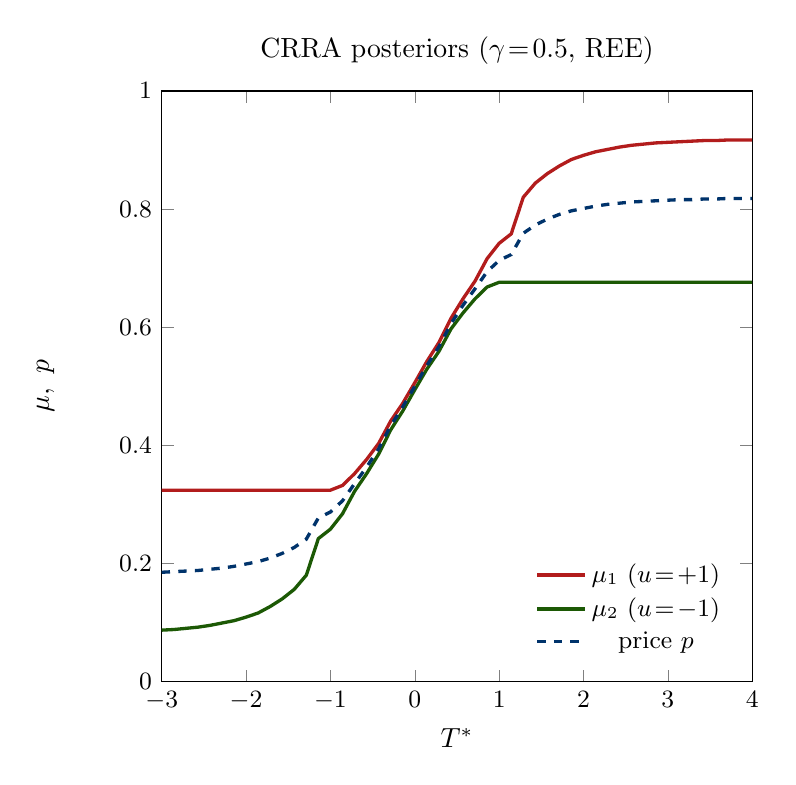
\begin{tikzpicture}
\begin{groupplot}[group style={group size=1 by 1}]
\nextgroupplot[
  xmin=-3, xmax=4,
  ymin=0, ymax=1,
  xlabel={$T^*$}, ylabel={$\mu,\; p$},
  legend pos=south east,
  title={CRRA posteriors ($\gamma\!=\!0.5$, REE)}]
% μ1 (agent 1, u=+1) — G=20 mp300
\addplot[very thick,color=BCred] coordinates {(-3.000,0.324)(-2.857,0.324)(-2.714,0.324)(-2.571,0.324)(-2.429,0.324)(-2.286,0.324)(-2.143,0.324)(-2.000,0.324)(-1.857,0.324)(-1.714,0.324)(-1.571,0.324)(-1.429,0.324)(-1.286,0.324)(-1.143,0.324)(-1.000,0.324)(-0.857,0.332)(-0.714,0.352)(-0.571,0.376)(-0.429,0.403)(-0.286,0.441)(-0.143,0.471)(0.000,0.506)(0.143,0.542)(0.286,0.574)(0.429,0.615)(0.571,0.648)(0.714,0.678)(0.857,0.716)(1.000,0.742)(1.143,0.758)(1.286,0.820)(1.429,0.844)(1.571,0.860)(1.714,0.873)(1.857,0.884)(2.000,0.891)(2.143,0.897)(2.286,0.901)(2.429,0.905)(2.571,0.908)(2.714,0.910)(2.857,0.912)(3.000,0.913)(3.143,0.914)(3.286,0.915)(3.429,0.916)(3.571,0.916)(3.714,0.917)(3.857,0.917)(4.000,0.917)};
% μ2 (agent 2, u=-1) — G=20 mp300
\addplot[very thick,color=BCgreen] coordinates {(-3.000,0.087)(-2.857,0.088)(-2.714,0.090)(-2.571,0.092)(-2.429,0.095)(-2.286,0.099)(-2.143,0.103)(-2.000,0.109)(-1.857,0.116)(-1.714,0.127)(-1.571,0.140)(-1.429,0.156)(-1.286,0.180)(-1.143,0.242)(-1.000,0.258)(-0.857,0.284)(-0.714,0.322)(-0.571,0.352)(-0.429,0.385)(-0.286,0.426)(-0.143,0.458)(0.000,0.494)(0.143,0.529)(0.286,0.559)(0.429,0.597)(0.571,0.624)(0.714,0.648)(0.857,0.668)(1.000,0.676)(1.143,0.676)(1.286,0.676)(1.429,0.676)(1.571,0.676)(1.714,0.676)(1.857,0.676)(2.000,0.676)(2.143,0.676)(2.286,0.676)(2.429,0.676)(2.571,0.676)(2.714,0.676)(2.857,0.676)(3.000,0.676)(3.143,0.676)(3.286,0.676)(3.429,0.676)(3.571,0.676)(3.714,0.676)(3.857,0.676)(4.000,0.676)};
% price (REE) — G=20 mp300
\addplot[very thick,color=BCblue,dashed] coordinates {(-3.000,0.185)(-2.857,0.186)(-2.714,0.187)(-2.571,0.188)(-2.429,0.190)(-2.286,0.192)(-2.143,0.195)(-2.000,0.199)(-1.857,0.203)(-1.714,0.209)(-1.571,0.217)(-1.429,0.227)(-1.286,0.241)(-1.143,0.277)(-1.000,0.287)(-0.857,0.306)(-0.714,0.335)(-0.571,0.363)(-0.429,0.394)(-0.286,0.433)(-0.143,0.465)(0.000,0.500)(0.143,0.535)(0.286,0.567)(0.429,0.606)(0.571,0.637)(0.714,0.665)(0.857,0.694)(1.000,0.713)(1.143,0.723)(1.286,0.759)(1.429,0.773)(1.571,0.783)(1.714,0.791)(1.857,0.797)(2.000,0.801)(2.143,0.805)(2.286,0.808)(2.429,0.810)(2.571,0.812)(2.714,0.813)(2.857,0.814)(3.000,0.815)(3.143,0.816)(3.286,0.816)(3.429,0.817)(3.571,0.817)(3.714,0.818)(3.857,0.818)(4.000,0.818)};
\legend{$\mu_1$ ($u\!=\!{+}1$), $\mu_2$ ($u\!=\!{-}1$), price $p$}
\end{groupplot}
\end{tikzpicture}
\end{document}
